\chapter{Formalización del problema}

El presente capítulo describe la estructura formal del problema de programación diaria del taller industrial,
incluyendo la caracterización del flujo operativo, la definición matemática de los elementos que componen el
sistema y la modelación del comportamiento del taller bajo sus restricciones reales. Los elementos
descriptivos del funcionamiento real del taller se documentan en el capítulo de Marco de Referencia;
aquí se retoman como insumo para la formulación matemática. Esta formalización constituye la base para
el desarrollo posterior del algoritmo genético y el método SPT, presentados en los capítulos siguientes.

\section{Estudio del flujo de trabajo del taller industrial}

El taller de reparación de motores opera bajo un flujo secuencial condicionado por restricciones de precedencia,
disponibilidad de repuestos, habilidades del personal e interacción entre tareas dentro de una misma orden
de trabajo. Cada día se recibe un conjunto de órdenes de trabajo que agrupan tareas mecánicas con distintos
requerimientos técnicos, y el objetivo operativo es completar la mayor cantidad posible de dichas tareas dentro
de la jornada laboral.

Operativamente, la jornada sigue el siguiente comportamiento conceptual:
\begin{enumerate}
    \item Llegan varias órdenes de trabajo, cada una con un conjunto de operaciones asociadas.
    \item Se identifican los recursos requeridos para cada operación: operarios aptos y repuestos específicos.
    \item Algunas tareas deben esperar a que otras concluyan dentro de una misma orden.
    \item Los operarios ejecutan las tareas secuencialmente dentro del horizonte diario disponible.
    \item Se prioriza maximizar el número de tareas completadas sin violar las restricciones operativas.
\end{enumerate}

Este flujo describe el contexto real que posteriormente se formaliza para alimentar la simulación y los algoritmos
 de optimización.

\subsection{Ejemplo de Estructura de Precedencias en una Orden Real}

La Figura~\ref{fig:precedencias-orden-real} muestra la estructura de dependencias de una orden de trabajo real del taller. Cada nodo representa una tarea con su identificador y nombre, mientras que las flechas direccionadas indican la relación de precedencia: una tarea solo puede iniciarse una vez que sus tareas predecesoras hayan sido completadas. Este tipo de restricciones son típicas en procesos de reparación de motores, donde ciertas operaciones (como pruebas de funcionamiento) deben realizarse al final, y otras (como rimar guías) pueden ejecutarse en paralelo siempre que no sea por el mismo operario. El diagrama ilustra cómo las restricciones de precedencia generan un grafo dirigido acíclico (DAG) que debe ser respetado durante la programación de las tareas.

\begin{figure}[H]
\centering
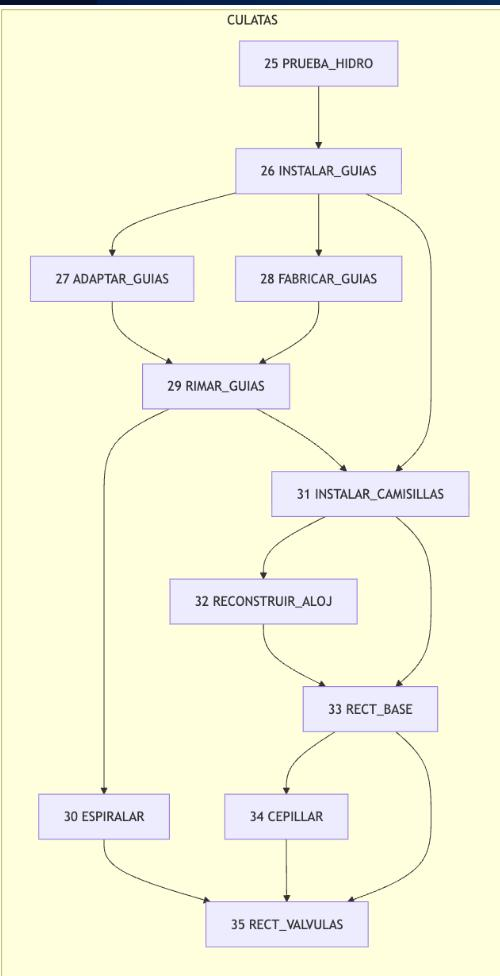
\includegraphics[width=0.65\textwidth]{figures/diagrama_tareas.jpg}
\caption{Estructura de precedencias de una orden de trabajo real del taller. Los nodos representan tareas identificadas por número y nombre, y las flechas indican relaciones de dependencia donde una tarea no puede iniciarse hasta que todas sus predecesoras hayan sido completadas. Este grafo dirigido acíclico es típico en procesos de reparación de motores.}
\label{fig:precedencias-orden-real}
\end{figure}

\section{Supuestos operativos y alcance}

Los supuestos del modelo parten de la caracterización levantada con el taller Recti-Ram. Se considera que:
\begin{itemize}
    \item La duración base de cada tipo de tarea es conocida y corresponde a tiempos promedio validados con expertos.
    \item Las habilidades de cada operario son estáticas durante la jornada y definen qué tareas puede ejecutar.
    \item Las precedencias sólo aplican dentro de una misma orden de trabajo.
    \item La disponibilidad de repuestos se conoce al inicio del día y se representa mediante parámetros binarios.
    \item Cada operario cuenta con un horizonte máximo de 480 minutos, equivalente a una jornada de 8 horas.
\end{itemize}

Estos supuestos delimitan el alcance del problema y sirven como base para la formalización matemática descrita a
continuación.

\section{Formalización Matemática del Problema}

\subsection{Conjuntos y parámetros fundamentales}

La estructura formal se define sobre los conjuntos:
\[
\begin{aligned}
OT &= \{1, \dots, m\} && \text{Órdenes de trabajo},\\
T_d &= \{1, \dots, n\} && \text{Tareas concretas del día},\\
O &= \{1, \dots, r\} && \text{Operarios disponibles},\\
T &= \{1, \dots, q\} && \text{Tipos de tarea identificados}.
\end{aligned}
\]

Los parámetros que caracterizan el sistema son:
\[
\begin{aligned}
p(t) &: T \rightarrow \mathbb{N} && \text{Duración base del tipo } t,\\
E(t) &\subseteq O && \text{Operarios aptos para el tipo } t,\\
P(t) &\subseteq T && \text{Tipos que deben preceder a } t,\\
R_{ot} &\in \{0,1\}^{|T|} && \text{Disponibilidad de repuestos por orden},\\
H &= 480 && \text{Horizonte diario en minutos}.
\end{aligned}
\]

Para cada tarea \(i \in T_d\) se conocen los parámetros \(ot(i) \in OT\) y \(tipo(i) \in T\).

\subsection{Variables de decisión y auxiliares}

La formalización utiliza el siguiente conjunto de variables:
\begin{itemize}
    \item \(x_i \in \{0,1\}\): indica si la tarea \(i\) se ejecuta dentro del horizonte.
    \item \(a_i \in O\): operario asignado a la tarea \(i\).
    \item \(s_i \geq 0\) y \(f_i = s_i + p(tipo(i))\): inicio y fin de la tarea \(i\).
    \item \(tpo_o \geq 0\): tiempo acumulado utilizado por el operario \(o\).
    \item \(comp_{ot}\): conjunto de tipos ya completados en la orden \(ot\).
    \item \(occ_{ot}\): conjunto de intervalos ocupados por tareas aceptadas dentro de la orden \(ot\).
\end{itemize}

Las tres últimas variables operan como estados auxiliares dentro de la simulación y permiten verificar factibilidad
al evaluar cada cronograma candidato.

\subsection{Estructura temporal}

El tiempo se modela como un intervalo continuo \([0, H]\). Cada tarea \(i\) programada por el operario \(a_i\) ocupa el
intervalo \([s_i, f_i)\), donde \(f_i = s_i + p(tipo(i))\). El tiempo acumulado por operario se actualiza mediante
\(tpo_{a_i} \gets f_i\) cuando se acepta la tarea, garantizando que la jornada individual no exceda \(H\).

\subsection{Restricciones operativas formales}

La factibilidad de una solución requiere cumplir simultáneamente las siguientes restricciones:
\begin{align}
a_i &\in E(tipo(i)) && \forall i \in T_d \label{cons:aptitud} \\
R_{ot(i)}(tipo(i)) &\geq x_i && \forall i \in T_d \label{cons:repuestos} \\
P(tipo(i)) &\subseteq comp_{ot(i)} && \forall i \in T_d \text{ con } x_i = 1 \label{cons:precedencia} \\
f_i &\leq H && \forall i \in T_d \label{cons:horizonte} \\
[s_i, f_i) &\cap occ_{ot(i)} = \emptyset && \forall i \in T_d \text{ con } x_i = 1 \label{cons:solape}
\end{align}

La restricción \eqref{cons:aptitud} garantiza que cada tarea se asigne a un operario competente, mientras que
\eqref{cons:repuestos} asegura la existencia de repuestos antes de iniciar la operación. La relación de precedencia
\eqref{cons:precedencia} obliga a que los tipos requeridos se encuentren en el conjunto de tareas completadas de la
misma orden. La cota temporal \eqref{cons:horizonte} impide exceder la jornada y \eqref{cons:solape} evita traslapos entre
tareas pertenecientes a la misma orden de trabajo.

Adicionalmente, la coherencia entre la variable binaria \(x_i\) y el cronograma se mantiene mediante las implicaciones:
\[
\begin{aligned}
x_i = 0 &\Rightarrow a_i \text{ y } s_i \text{ quedan sin asignar},\\
x_i = 1 &\Rightarrow s_i = tpo_{a_i}, \quad f_i = s_i + p(tipo(i)).
\end{aligned}
\]

\subsection{Definición formal del problema de optimización}

El objetivo operativo consiste en maximizar el número de tareas completadas durante la jornada, lo cual se expresa como:
\[
\begin{aligned}
\max_{x,a,s} \quad & \sum_{i \in T_d} x_i \\
\text{s.a.} \quad & \text{Restricciones \eqref{cons:aptitud}--\eqref{cons:solape}}, \\
& x_i \in \{0,1\}, \; a_i \in O, \; s_i \geq 0, \quad \forall i \in T_d.
\end{aligned}
\]

La solución del problema proporciona un cronograma factible que respeta las reglas industriales y utiliza de forma
 eficiente la capacidad diaria disponible.

\section{Representación computacional del sistema}

Para ejecutar la simulación y alimentar los algoritmos, la formalización anterior se implementa mediante una
configuración digital que integra todos los elementos estructurales del taller:
\begin{itemize}
    \item \textbf{Catálogo de tareas}: lista de los tipos contenidos en \(T\), cada uno con su duración base \(p(t)\) y la
    familia operativa correspondiente.
    \item \textbf{Matriz de habilidades}: representación explícita de \(E(t)\), indicando qué operarios están calificados para
    cada tipo de tarea.
    \item \textbf{Relaciones de precedencia}: estructuras de datos que codifican \(P(t)\) y permiten validar dependencias dentro
    de una misma orden.
    \item \textbf{Parámetros diarios}: conjunto de tareas \(T_d\), asociación con órdenes \(ot(i)\) y disponibilidad de repuestos
    \(R_{ot}\) derivada del levantamiento de información real.
    \item \textbf{Horizonte y estados auxiliares}: valores iniciales de \(tpo_o\), \(comp_{ot}\) y \(occ_{ot}\) que se actualizan
    durante la evaluación de cada solución.
\end{itemize}

Esta representación computacional garantiza consistencia entre la formalización matemática y el comportamiento del
simulador que se utiliza en los capítulos posteriores para evaluar SPT y el algoritmo genético.
